\documentclass[parskip=half]{scrartcl}

\usepackage{tabu}
\usepackage{amsmath}
\usepackage{mathtools}
\usepackage{graphicx}
\usepackage{hyperref}
\graphicspath {{images/}}
\hypersetup{
    colorlinks=true,
    citecolor=blue
}

\begin{document}

\title{CS798 (Winter 2017) Notes}
\author{Vineet John (v2john@uwaterloo.ca)}
\date{}
\maketitle

\section{Chord} % (fold)
\label{sec:chord}

    \subsection{Chord Overview} % (fold)
    \label{sub:chord_overview}

    \begin{itemize}
        \item
        Chord is a distributed P2P lookup protocol. It helps locate the node storing any given data.
        \item
        USP is that it deals with frequent node arrivals and departures.
        \item
        The Chord protocol supports \textbf{just one operation: given a key, it maps the key onto a node.}
        \item
        Consistent hashing is used to balance the storage for the nodes. (Normalizing the bucket contents)
        \item
        Each Chord node needs routing information about only a few other nodes. Because the routing table is distributed, a node resolves the hash function by communicating with a few other nodes.
        \item
        Key problems addressed: Load balance, decentralization, scalability, availability and flexible naming
    \end{itemize}

    % subsection overview (end)

    \subsection{Chord Implementation} % (fold)
    \label{sub:chord_implementatio}
    \begin{itemize}
        \item
        Routing information about only $O(log n)$ other nodes are maintained at each node.
        \item
        Chord provides a lookup(key) algorithm that yields the IP address of the node responsible for the key.
        \item
        The Chord software on each node notifies the application of changes in the set of keys that the node is responsible for.
        \item
        In an N-node network, a lookup requires $O(log n)$ messages. A join or leave from the network requires $O(log^2 n)$ messages.
        \item
        Both nodes and keys are given an identifier $m$ bits in length.  Identifiers are ordered in an identifier circle modulo $2^m$. Key is assigned to the first node whose identifier is equal to or follows (the identifier of) $k$ in the identifier space. This node is called the successor node of key $k$, denoted by $successor(k)$ . If identifiers are represented as a circle of numbers from 0 to $2^m - 1$, then $successor(k)$ is the first node clockwise from $k$.\\
        This lets nodes enter and leave with minmal disruption.  To maintain the consistent hashing mapping when a node $n$ joins the network, certain keys previously assigned to $n's$ successor now become assigned to $n$. When node $n$ leaves the network, all of its assigned keys are reassigned to $n's$ successor.
        \item
        \textbf{Consistent hashing theorem}
        \begin{itemize}
            \item
            Each node is responsible for at most $\frac{(1 + \epsilon) K}{N}$ keys
            \item
            When a node joins/leaves the network responsibility of $O(\frac{K}{N})$ changes hands from/to the node in question.
        \end{itemize}
        \item
        \textbf{Finger tables} are used to maintain information about $log(N)$ successors. This isn't needed for correctness. Every node could just have information about it's successor, but then the complexity of a lookup would be $O(N)$\\
        For a node $n$, it's finger nodes would be at $(n + 2^{k-1}) \mod 2^m$, where $1 \leq k \leq m$, within the identity circle.
        \item
        Data possessed by a single node in the Chord cluster:\\
        \begin{tabular}{|| c | c ||}
        \hline\hline
        \textbf{Notation} & \textbf{Definition} \\
        \hline\hline
        $finger[k].start$  &  $(n + 2^{k-1}) \mod 2^m$, where $1 \leq k \leq m$\\
        \hline
        $.interval$  &  $finger[k].start, finger[k+1].start$\\
        \hline
        $.node$  &  first node $\geq n.finger[k].start$\\
        \hline
        $successor$  &  the next node on the identifier circle $\geq finger[1].node$\\
        \hline
        $predecessor$  &  the previous node on the identifier circle\\
        \hline\hline
        \end{tabular}
        \item
        The \textbf{Join algorithm} picks an arbitrary node and adds itself as it's successor. It then creates it's own finger tables and other variables, and then updates the other nodes that need to have the new node in their finger tables.
        \item
        \textbf{Stabilization} does 2 things after the join algorithm. It stabilizes the new node by notifying it's successor about the fact that it succeeds the new node. It also periodically refreshes finger table entries.
        \item
        \textbf{Failures:} Rather than maintaining just a single successor, each node has a list of successors to fall back on in case the immediate successor goes down.

    \end{itemize}

    % subsection how_it_works (end)

    \subsection{Use-Cases} % (fold)
    \label{sub:use_cases}

    \begin{itemize}
        \item
        Co-operative Mirroring: Devs hosting different distributions across multiple nodes.
        \item
        Time-shared storage: Host content for others while up, let others host content for you when down.
        \item
        Distributed Indices
        \item
        Large-scale Combinatorial Search
    \end{itemize}

    % subsection use_cases (end)

% section chord (end)
\newpage

\section{Dynamo} % (fold)
\label{sec:dynamo}

    \subsection{Dynamo Overview} % (fold)
    \label{sub:dynamo_overview}
    \begin{itemize}
        \item
        Key-value store. Availability and reliability are important.
        \item
        Data is partitioned and replicated using consistent hashing. (storage balancing)
        \item
        Consistency among replicas during updates maintained by a quorum-like technique and a decentralized replica synchronization protocol
        \item
        Eventually consistent system. Gossip based failure failure detection and membership.
        \item
        CAP theorem: Consistency traded for high availability and partition tolerance, in the event of failures.
        \item
        Conflict resolution of inter-node inconsistency is resolved by reads, not writes. Writes need to be highly-available. (Shopping cart analogy.)
        \item
        No authoritative node a.k.a. leader
    \end{itemize}

    % subsection overview (end)

    \subsection{Dynamo Implementation} % (fold)
    \label{sub:dynamo_implementation}

    \begin{itemize}
        \item
        MD5 hash for consistent hashing - to locate partition to store in. 128-bit hash identifier for each key.
        \item
        Output range of the \textbf{consistent hash function} is treated as a \textbf{fixed circular space or “ring”} (i.e. the largest hash value wraps around to the smallest hash value)
        \item
        Partitioning similar to Chord's. Departure and arrival of nodes only affect their immediate successors on the ring.
        \item
        Virtual nodes used to assign physical nodes to multiple places on the ring. Deviation from consistent hashing. A single physical node can map to multiple virtual nodes. Virtual nodes help evenly disperse the load of a single physical node going down.
        \item
        A node replicates keys with a factor of N. Apart from it's own copy, it places a copy on each of the `N' nodes that follow it. The list of nodes designated for a key is called a \textbf{preference list}.
        \item
        get() and put() are the available functions.
        \item
        get() returns either a single value or a list of conflicting values along with a context object.
        \item
        put() accepts a key, value and a context object. The context is opaque to the caller.
        \item
        Versioning helps with maintaining multiple immutable versions of the same object.
        \item
        \textbf{Vector clocks} used to determine causality of object versions. A vector clock is a list of (node, counter) pairs. eg. $[(S_x,3), (S_y, 1), (S_z, 1)]$. Dynamo adds a timestamp to this pair, and truncates the oldest pairs from the vectors once it reaches a certain
        \item
        Clients reconcile divergent versions of the same object.
        \item
        Quorum consistency protocol used. $R + W > N$. N, R and W can be tuned client-side.
        \item
        \textbf{Hinted handoff}. Sloppy quorum. In case of unavailability of the N highest-ranked reachable nodes, send update to the first N healthy nodes.
        \item
        Replica synchronization. \textbf{Merkle trees used to detect inconsistencies between replicas}. A Merkle tree is a hash tree where leaves are hashes of the values of individual keys. Parent nodes higher in the tree are hashes of their respective children. Helps avoid unnecessary checking if the root of the tree has a similar hash to it's replica.
        \item
        However, if a node is added/removed, then all Merkle trees need to be recomputed, because key-ranges will change.
        \item
        Gossip-based membership.  Each node contacts a peer chosen at random every second and the two nodes efficiently reconcile their persisted membership change histories
        \item
        Each storage node has three main software components: request coordination, membership and failure detection, and a local persistence engine.
        \item
        Request co-ordination implemented in a \textbf{SEDA style. Event and stage-driven requests}.
        \item
        Buffers used as a caching layer, and also to delay persisting writes. Buffer written on multiple W nodes for quorum.
        \item
        Each incoming request handled by a state-machine specific to it. Contains all the context needed for the request.
        \item
        Latency metrics show that client-based co-ordination is more beneficial that server-based. No load balancer needed.
        \item
        Each node knows about every other node i.e. complete routing table, through the gossip based protocol. (Seed nodes are the initial nodes that a new node will know about in a cluster). $O(1)$ routing.
        \item
        In figure \ref{fig:dynamo-consensus}, if Paxos or Raft acted on the majority half, they would've succedded, but if not, they would've failed. Dynamo doesn't need to write to a majority for the write to have been logged.
        \begin{figure}[th]
            \centering
            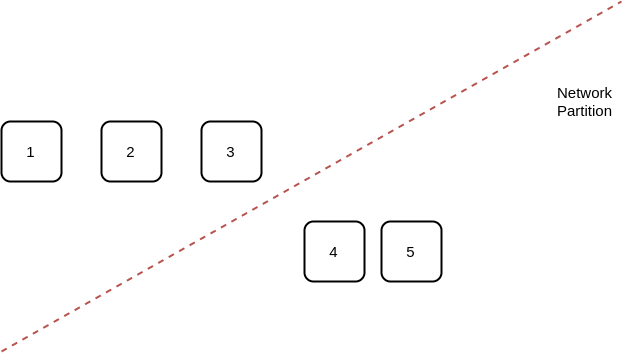
\includegraphics[width=.5\textwidth]{dynamo-consensus}
            \caption{Consensus with Quorum}
            \label{fig:dynamo-consensus}
        \end{figure}
        \item
        Gossip protocol working
        \begin{itemize}
            \item
            Pick random node
            \item
            Exchange membership info
        \end{itemize}
        \item
        Background tasks are limited to a threshold.
    \end{itemize}

    % subsection dynamo_implementation (end)

    \begin{figure}[th]
    \centering
    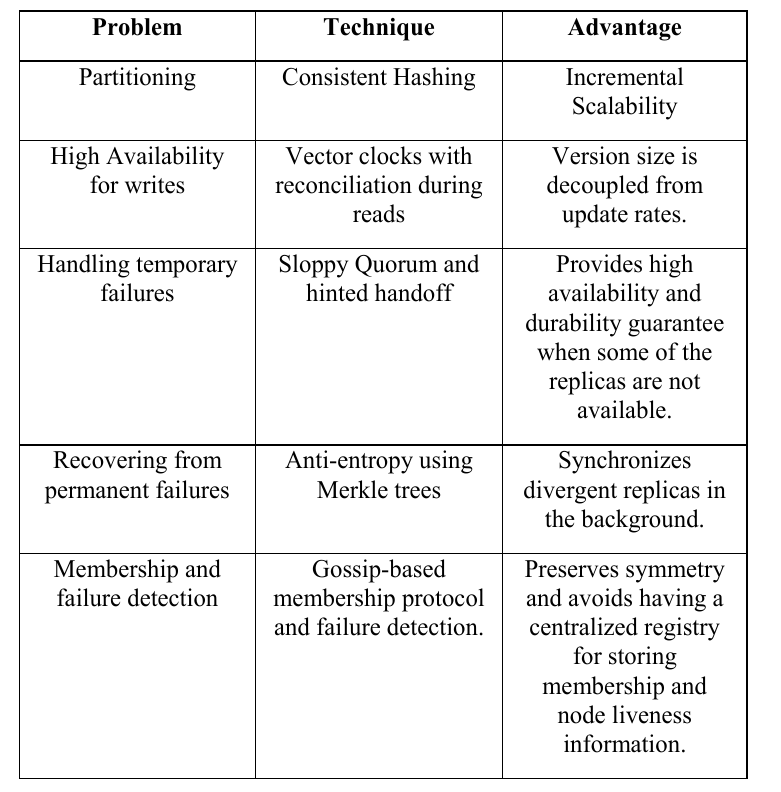
\includegraphics[width=.5\textwidth]{dynamo-techniques}
    \caption{Techniques and Advantages}
    \label{fig:dynamo-techniques}
    \end{figure}

% section dynamo (end)

\newpage

\section{Live Migration of VMs} % (fold)
\label{sec:live_migration_of_vms}

    \subsection{Motivation - Virtualization} % (fold)
    \label{sub:motivation_virtualization}

        \begin{itemize}
            \item Maintenance
            \item Load Management (Balancing/Consolidation)
        \end{itemize}

        Problems to tackle in terms of complexity:
        \begin{itemize}
            \item Need to handle memory, disk, file system, IPC, sockets.
            \item Higher overhead ($5\%$ overhead nowadays)
        \end{itemize}

    % subsection motivation_virtualization (end)

    \subsubsection{VM Migration - Overview} % (fold)
    \label{ssub:vm_migrationn_overview}

        \textbf{Goal:}
        \begin{itemize}
            \item Reduce the time that the VM isn't available i.e. reduce downtime.
            \item Reduce the time for migration i.e. until the former host can be decommissioned.
        \end{itemize}

        \begin{figure}[th]
            \centering
            \includegraphics[width=0.6\textwidth]{vm-arch}
            \caption{VM Architecture}
            \label{fig:vm-arch}
        \end{figure}

        \textbf{Approaches:}
        \begin{itemize}
            \item Stop-and-copy. (Results in high downtime)
            \item Copy-on-demand. First copy the kernel state. Rest of memory copied on page faults on the new system. (Low downtime, but indefinitely high migration time)
            \item Pre-copy:
            \begin{itemize}
                \item Select a target node.
                \item Allocate resources (Memory, BLK devices).
                \item Copy all memory to the target node.
                \item While copying, keep track of the changes made to the memory on the source node. (dirty pages). Do this iteratively until a lower bound on the number of dirty pages on each iteration is reached, and then do a stop-and-copy.
                \item Redirect network traffic to the target node.
                \item Target node is activated and the source node is discarded.
            \end{itemize}
        \end{itemize}

        \textbf{Failure:} Not worse that the null hypothesis, where the decision to migrate is not even taken.

        \textbf{Storage:} Both nodes can utilize a NAS for storage, which will eliminate the need to physically copy memory pages from one node to the other.

        \textbf{Network:} VM network stack is migrated and IP address is maintained.
        \begin{itemize}
            \item Send ARP update to announce the re-allocation of the source node IP address. i.e. Change the MAC address associated with the IP address.
            \item In-flight packets are lost. This is supposed to be handled by the application's chosen communication protocol, or by the application itself.
        \end{itemize}

        \textbf{Optimizations:}
        \begin{itemize}
            \item Dynamic Rate Limiting: Trade-off between contention and migration time.
            \item Avoid copying frequently dirtied pages by peeking.
            \item Limit processes that dirty a lot of pages.
            \item Avoid copying free pages.
        \end{itemize}

        \textbf{Across DC Migration:}
        \begin{itemize}
            \item Lower B/W and Higher latency.
            \item Migrate disk.
            \item Dependencies on other VMs need to be migrated.
            \item Dependencies on the DC itself, if applicable, need to be migrated.
        \end{itemize}

        \textbf{Misc:}
        \begin{itemize}
            \item Xen VMM is the platform used for the study. Live migration with downtimes as low as 60ms is the USP.
            \item The narrow interface between a virtualized OS and the virtual machine monitor (VMM) makes it easy avoid the problem of ‘residual dependencies’.
            \item Virtualization allows for a transfer of in-memory state consistenty and efficiently and provides a separation between the users and the service providers. The service providers can remain agnostic to the content and processes inside a particular VM unit while migrating it.
        \end{itemize}

    % subsubsection vm_migrationn_overview (end)

% section live_migration_of_vms (end)

\newpage

\section{Remus} % (fold)
\label{sec:remus}


    \subsection{Remus - Overview} % (fold)
    \label{sub:remus_overview}

        \begin{itemize}
            \item High-availability VMs. Meant to be used for asynchronous VM replication.
            \item Hides failures: failures look like lost packets to a client
        \end{itemize}

    % subsection remus_overview (end)

    \begin{figure}[th]
        \centering
        \includegraphics[width=0.6\textwidth]{remus-arch}
        \caption{Remus Architecture}
        \label{fig:remus-arch}
    \end{figure}

    \subsection{Remus - Working} % (fold)
    \label{sub:remus_working}

        \begin{itemize}
            \item During an epoch, client requests are served by the primary node, response is buffered.
            \item At the end of an epoch, pause primary VM and stop-and-copy dirtied pages to backup.
            \item Resume primary node.
            \item Asynchronous part is release the buffers to disk, and releasing updates to the cient
        \end{itemize}

    % subsection remus_working (end)


% section remus (end)

\newpage


\section{Petal - Distributed Virtual Disks} % (fold)
\label{sec:petal_distributed_virtual_disks}

    \begin{itemize}
        \item
        N/W of servers co-operatively managing a pool of disks.
        \item
        To a client, Petal appears to be a block storage system with abstract containers. Clients are permitted create of virtual disks on demand. Client view: Figure \ref{fig:petal-client-view}.
        \begin{figure}[ht]
            \centering
            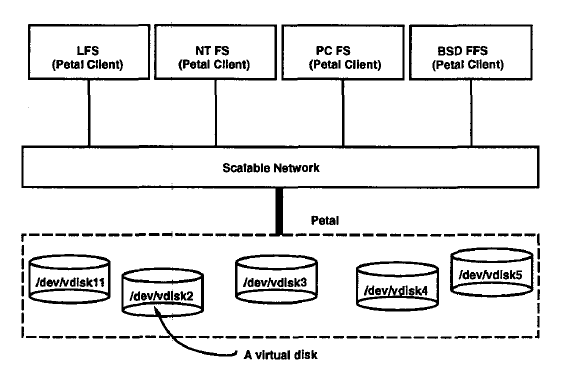
\includegraphics[width=.4\textwidth]{petal-client-view}
            \caption{Petal Client View}
            \label{fig:petal-client-view}
        \end{figure}
        \item
        Can tolerate and recover from disk, network and storage failures. Can be geographically distributed.
        \item
        Transparently reconfigures to enhance or degrade performance based on addition or removal of nodes to the cluster.
        \item
        Load balancing is universal. Backup and recovery supported.
        \item
        Physical view: Figure \ref{fig:petal-physical-view}
        \begin{figure}[ht]
            \centering
            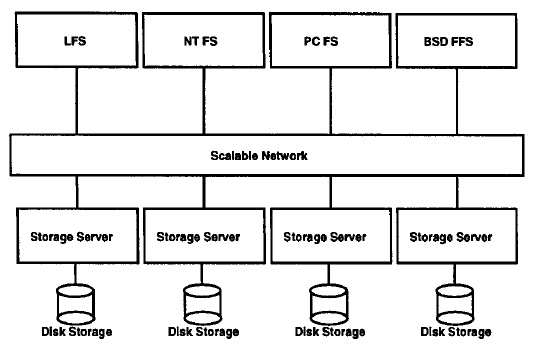
\includegraphics[width=.4\textwidth]{petal-physical-view}
            \caption{Petal Physical View}
            \label{fig:petal-physical-view}
        \end{figure}
        \item
        Petal services are accessed via RPC.
        \item
        State maintained on the servers for integrity. Clients only posses hints about which servers to connect for a given address range.
        \item
        Petal Modules: Figure \ref{fig:petal-server-modules}
        \begin{figure}[ht]
            \centering
            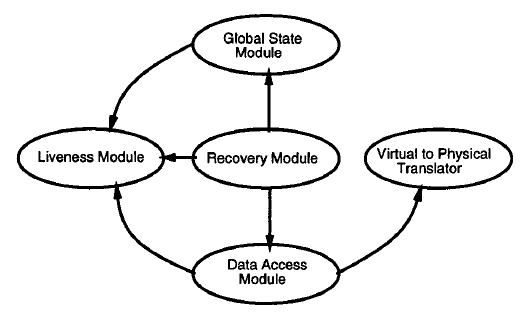
\includegraphics[width=.4\textwidth]{petal-server-modules}
            \caption{Petal Server Modules}
            \label{fig:petal-server-modules}
        \end{figure}
    \end{itemize}

    \subsection{Considerations} % (fold)
    \label{sub:considerations}
    
        \begin{itemize}
            \item 
            Data consistency
            \item 
            Address translation
            \item 
            Reconfiguration
            \item 
            Recovery
            \item 
            Backup
        \end{itemize}

    % subsection considerations (end)

    \subsection{Petal - Design} % (fold)
    \label{sub:petal_design}

        \begin{itemize}
            \item
            Servers maintain most of the state for data integrity.
            \item
            Information about the current member of the storage system is replication across all the Petal servers.
            \item
            Global State Manager maintains the state information. Consensus for members (nodes) is arrived at using Paxos. (Part-time parliament) This guarantees progress as long as a majority of the nodes are in agreement.
            \item
            Clients interact with Petal via the data access module.
            \item
            Level of redundancy of the data is config-driven. The redundancy scheme used is \textbf{Chained Declustering}.
            \item
            Virtual to Physical address translation needs to be done by the Virtual Disk Directory.\\
            \texttt{<virtual-disk-id, offset> = <server-id, physical-disk-id, offset>}
            \item 
            3 Main Data-structures are used for the translation of a virtual address into the physical address space:
            \begin{itemize}
                \item 
                Virtual disk directory: Translate client supplied virtual identifier to a Global Map ID.
                \item 
                Global map identifier: Identifies the server responsible for a given offset.
                \item 
                Physical map: GMI and offset are translated into a physical offset.
            \end{itemize}
            \item 
            Gmap is immutable.
            \item 
            Typically, steps 2 and 3 are performed by the same server. If the client has a reliable hint about which server to contact, then all the steps can be carried out by a single Petal server.
        \end{itemize}

    % subsection petal_design (end)

    \subsection{Petal - Backup} % (fold)
    \label{sub:petal_backup}

        \begin{itemize}
            \item 
            Snapshots of the virtual disks are used as backup.
            \item 
            Epochs are used to distinguish data written at different points in time.
            \item 
            Copy-on-write techniques used for backup. This means that the clients read from the same version of the data, but if they have to write to the data, they get their own copy.
            \item 
            When a backup is created, a new data tuple of \texttt{<global-map-identifier, epoch>} is created. The old one is used for the snapshot, and the new one is used for future requests.
        \end{itemize}
    
    % subsection petal_backup (end)

    \subsection{Petal - Virtual Disk Reconfiguration} % (fold)
    \label{sub:petal_virtual_disk_reconfiguration}

        \begin{itemize}
            \item 
            Need to handle the resources arriving or leaving the Petal cluster.
            \item 
            Addition of a disk to a server is handled locally by that server.
            \item 
            Addition of a server is more complex and comprises of:
            \begin{itemize}
                \item 
                Needs to be added as a member of the storage system.
                \item 
                Liveness monitor needs to include the new server.
                \item 
                Existing virtual disks to utilize the new server.
            \end{itemize}
            \item 
            The process for virtual disk reconfig. is as follows:
            \begin{itemize}
                \item 
                Create new global map with redundancy scheme and server mapping.
                \item 
                Change all the virtual disk entries to point to the new global map.
                \item 
                Redistribute data based on the new address translation scheme.
            \end{itemize}
            \item 
            Data is moved starting with the most recent epoch. This ensures that client reads do not return out of data.
            \item 
            If an address is unavailable from the new global map, then query the old global map. This is inefficient especially immediately after the change is made from the old to the new global map.
            \item 
            Refined algorithm:
            \begin{itemize}
                \item 
                Split the address space into three regions: \texttt{old}, \texttt{fenced} and \texttt{new}.
                \item 
                If the address space requested is from the \texttt{old} or \texttt{new} regions, serve them from the corresponding global maps. If the address space is from the \texttt{fenced} region, then fall back to the earlier algorithm, which first checks the new global map, and then the old if the address is not found.
            \end{itemize}
            \item 
            The idea of the refined algorithm is to keep the fenced region small, and permit lesser `cache misses'.
        \end{itemize}
    
    % subsection petal_virtual_disk_reconfiguration (end)

    \subsection{Petal - Data Access and Recovery} % (fold)
    \label{sub:petal_data_access_and_recovery}

        \begin{itemize}
            \item 
            Chained declustering is used. Ref Figure \ref{fig:petal-chained-declustering}
            \begin{figure}[ht]
                \centering
                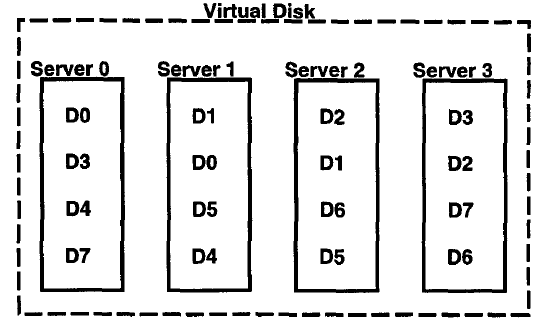
\includegraphics[width=.4\textwidth]{petal-chained-declustering}
                \caption{Petal Chained Declustering}
                \label{fig:petal-chained-declustering}
            \end{figure}
            \item 
            If Server 0 goes down in the architecture presented in figure \ref{fig:petal-chained-declustering}, servers 1 and 3 have a combined backup of the data. Hence the load is rebalanced to these two servers, but not Server 2. However, Servers 1 and 3 can delegate additional load responsibilities to Server 2 for the data elements that they co-own.
            \item 
            This is called \textbf{striping}.
            \item 
            Supposedly less reliable than simple mirroring, since either of Server 1 or 3 going down will mean a complete loss of certain data.
        \end{itemize}
    
    % subsection petal_data_access_and_recovery (end)

    \subsection{Petal - Data Access Semantics} % (fold)
    \label{sub:petal_data_access_semantics}

        \textbf{Reads}
        \begin{itemize}
            \item 
            Client makes a request
            \item 
            If the server is able the read the data locally, the data is returned.
            \item 
            Else the server returns an error code.
            \item 
            Client tries another server if it receives an error code.
        \end{itemize}

        \textbf{Writes:}\\
        Different from reads in that the behavior is different if the primary data owner node is down.
        \begin{itemize}
            \item 
            Primary Copy Available
            \begin{itemize}
                \item 
                Sets a busy bit for the addresses in question
                \item 
                Propagates the changes both locally and to the replicated node.
                \item 
                Once the write is confirmed, the busy bits are cleared.
                \item 
                Busy bits cached for quicker access.
            \end{itemize}
            \item 
            Primary Copy Unavailable
            \begin{itemize}
                \item 
                Write request is directed to a backup node.
                \item 
                Node verifies that the primary is unavailable.
                \item 
                It sets the data element as stale and updates the local disk.
                \item 
                Once the primary node is back up, it needs to resolve it's local disk for the entries that have been marked as stale.
            \end{itemize}
        \end{itemize}
    
    % subsection petal_data_access_semantics (end)

    \subsection{Petal - Implementation, Performance and Misc} % (fold)
    \label{sub:petal_implementation_performance_and_misc}

        \begin{itemize}
            \item 
            RPC calls for the Petal API are mostly virtual disk management related.
            \item 
            Throughput scales with an increased number of servers.
            \item 
            Most other solutions use single node metadata node driven-architectures.
            \item 
            Block level data interface preferred over a filesystem interface in Petal.
        \end{itemize}
    
    % subsection petal_implementation_performance_and_misc (end)

% section petal_distributed_virtual_disks (end)


\newpage


\section{Frangipani - Scalable Distributed File System} % (fold)
\label{sec:frangipani_scalable_distributed_file_system}

    \begin{itemize}
        \item 
        Distributed File System built with the lower layer as Petal.
        \item 
        Needs a distributed lock system to function.
        \item 
        Meant to be run on a cluster under a common administration and communicate securely.
        \item 
        The cluster comprises a set of co-operating machines with a common datastore. Data element access is synchronized using the locking service.
        \item 
        All users see a consistent view of the file system. There is a separation of concerns between the users and the ownership of their data.
        \item 
        Server addition is flexible.
        \item 
        Live backups can be initiated.
        \item 
        Similar to Petal, Frangipani can survive N/W, server and disk failures.
        \item 
        The implementation extends the underlying Petal's block-type system to a file-system.
    \end{itemize}

    \subsection{Frangipani - Structure} % (fold)
    \label{sub:frangipani_structure}
    
        \begin{itemize}
            \item 
            Layering Architecture: Figure \ref{fig:frangipani-layering}
            \begin{figure}[ht]
                \centering
                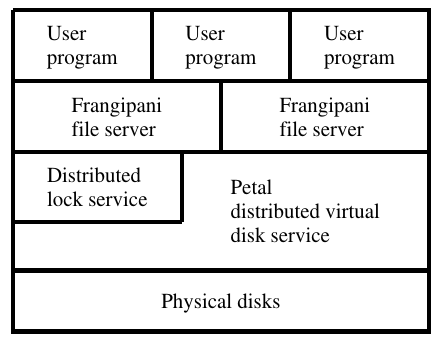
\includegraphics[width=.4\textwidth]{frangipani-layering}
                \caption{Frangipani Layering}
                \label{fig:frangipani-layering}
            \end{figure}
            \item 
            Describes as a cluster file-system.
            \item 
            Frangipani Structure: Figure \ref{fig:frangipani-structure}
            \begin{figure}[ht]
                \centering
                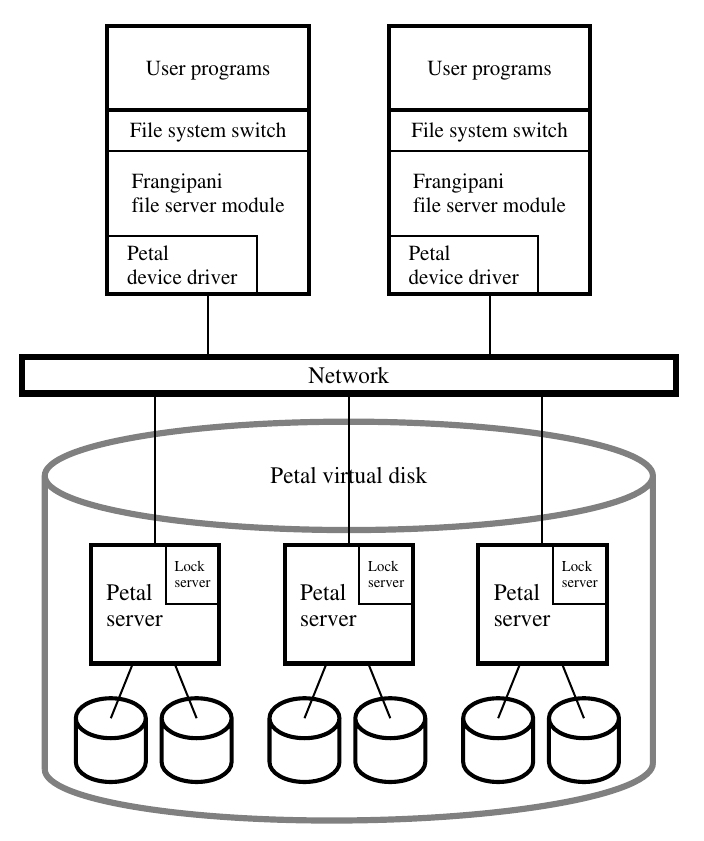
\includegraphics[width=.4\textwidth]{frangipani-structure}
                \caption{Frangipani Structure}
                \label{fig:frangipani-structure}
            \end{figure}
            \item 
            File server module (Figure \ref{fig:frangipani-structure}) runs within the OS kernel.
            \item 
            Retains last accessed metadata of data elements approximately.
            \item 
            Petal device driver used to write to the physical Petal nodes.
            \item 
            FP servers don't communicate with each other - only with Petal and the lock service.
            \item 
            FP registers with the kernel file-system switch as one of the available file systems.
            \item 
            Petal device driver makes the distributed file system seem local.
            \item 
            Lock service used for multiple reader, single writer access across the system.
            \item 
            Security measures - Petal servers accept requests only from whitelisted FP servers.
            \item 
            Untrusted clients can use FP servers as a proxy as show in Figure \ref{fig:frangipani-client-server}. This can be done using NFS/SMB or similar remote file-system access protocols.
            \begin{figure}[ht]
                \centering
                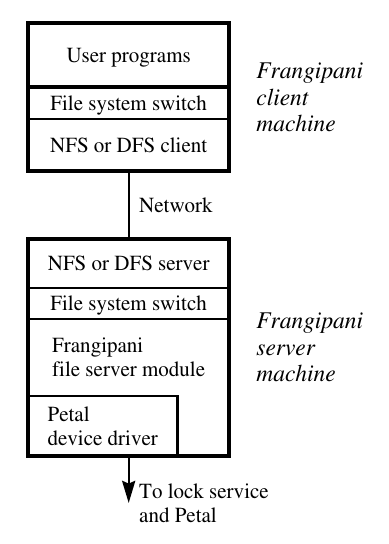
\includegraphics[width=.4\textwidth]{frangipani-client-server}
                \caption{Frangipani Client-Server}
                \label{fig:frangipani-client-server}
            \end{figure}
            \item 
            The access semantics for Frangipani are filesystem like, rather than disk-like, as opposed to Petal.
        \end{itemize}

    % subsection frangipani_structure (end)

    \subsection{Frangipani - Disk Layout} % (fold)
    \label{sub:frangipani_disk_layout}
    
        \begin{itemize}
            \item 
            Petal Virtual Disk comprises $2^{64}$ bytes of address space.
            \item 
            5 segments of the disk layout are:
            \begin{itemize}
                \item 
                Config and housekeeping
                \item 
                Logs that are partitioned
                \item 
                Allocation bitmaps - metadata about storage being free. Each server owns a portion of the bitmap.
                \item 
                Inodes - symbolic links and small files are self contained within inodes.
                \item 
                Small data blocks. Larger files than 64kb are stored in larger blocks.
            \end{itemize}
        \end{itemize}

    % subsection frangipani_disk_layout (end)

    \subsection{Frangipani - Logging and Recovery} % (fold)
    \label{sub:frangipani_logging_and_recovery}

        \begin{itemize}
            \item 
            Write-ahead redo-logging is used. i.e. logging takes place prior to an action being performed, so that the log can be replayed in the event of a failure immediately after the log is written.
            \item 
            Each FP server maintains a log in Petal. The append RPCs to Petal could be synchronous if failure recovery is a lot more important to the system than metadata write latency.
            \item 
            Circular buffer used for logging. The oldest 25\% is reclaimed once the buffer is full. It has monotonously increased IDs. This helps detect where the start of the buffer is.
            \item 
            Recovery daemon accesses the failed FP servers logs from Petal. It makes the necessary updates written to the log, and releases the locks. During recovery, write only blocks with version numbers larger than the current version number on disk.
            \item 
            For any given block in Petal, at most one FP log can possess an update lock for it.
            \item 
            Only metadata is logged, not user data. Hence, failures post recovery are visible to the users.
        \end{itemize}
    
    % subsection frangipani_logging_and_recovery (end)

    \subsection{Frangipani - Cache Coherence} % (fold)
    \label{sub:frangipani_cache_coherence}

        \begin{itemize}
            \item 
            A read lock allows a server to cache the data that it acquired the lock for. If requested to relinquish the lock, the server needs to invalidate it's cache before doing so.
            \item 
            The FP server and the disk version of the data can only be different if the FP server holds a write lock on the data. If such a server is requested to downgrade or relinquish it's lock, it must ensure that the dirty data that is present locally is flushed to Petal(disk) before doing so.
        \end{itemize}
    
    % subsection frangipani_cache_coherence (end)

    \subsection{Frangipani - Locking} % (fold)
    \label{sub:frangipani_locking}

        \begin{itemize}
            \item 
            Single Writer, Multiple Reader.
            \item 
            Locks are sticky i.e. retained until requested by another server.
            \item 
            Locks are also lease based (???)
            \item 
            Options evaluated for locking in Frangipani:
            \begin{itemize}
                \item 
                Locking service
                \item 
                Lock state maintained on a Petal virtual disk
                \item 
                Distributed lock servers, with a clerk used as an intermediary to communicate with Frangipani servers. In this scenario, the lock state is replicated using Paxos.
            \end{itemize}
            \item 
            When an FP server crashes, the locks that it held cannot simply be released, since it may have pending updates. This is handled by the recovery daemon.
            \item 
            Requests from FP servers with imminent lease expiry are not handled in FP, but the handling could be as simple as timestamping the point of expiry, and allow Petal to discard out-of-date requests, or by using a lease identifier at the Petal servers.
            \item 
            FP uses file-level locking, which is described as being coarse-grained.
        \end{itemize}
    
    % subsection frangipani_locking (end)

    \subsection{Frangipani - Adding or Removing Servers} % (fold)
    \label{sub:frangipani_adding_or_removing_servers}

        \begin{itemize}
            \item 
            No requirement to inform or access other FP servers during addition. The new server just needs to be aware of the Petal service and the locking service.
            \item 
            For removal, an FP server can just be turned off, since the recovery daemon can handle it's unwritten updates to disk.
        \end{itemize}
    
    % subsection frangipani_adding_or_removing_servers (end)

    \subsection{Frangipani - Backup} % (fold)
    \label{sub:frangipani_backup}

        \begin{itemize}
            \item 
            FP relies on Petal for backup, via Petal's snapshotting feature.
            \item 
            If needed a backup can also be made filesystem compatible. This can be done by gradually entering all the FP servers into a barrier state and then triggering a Petal snapshot. This snapshot can then directly be mounted as a filesystem.
            \item 
            Both these techniques result in snapshots that are read-only, since that is how Petal has implemented it.
        \end{itemize}
    
    % subsection frangipani_backup (end)

    \subsection{Frangipani - Performance} % (fold)
    \label{sub:frangipani_performance}

        \begin{itemize}
            \item 
            Performance can be boosted by adding an NVRAM buffer in front of the disk in Petal. This is presumably because logging will be faster, and so with updates to the disk.
            \item 
            Throttling was noticed due to read-ahead and lock-contention, causing the readers to frequently invalidate their caches when the lock ownership is being passed around in a round-robin manner.
            \item 
            Justification for locking at file-level is the workloads that FP is designed for.
        \end{itemize}

    % subsection frangipani_performance (end)

% section frangipani_scalable_distributed_file_system (end)


\newpage


\section{Authentication} % (fold)
\label{sec:authentication}

    \begin{itemize}
        \item 
        \textbf{Secure communication}
        \begin{itemize}
            \item 
            Integrity: no modification done to the message by intruders
            \item 
            Confidentiality: secrecy i.e. message not readable by intruders.
            \item 
            Authenticity: users are who they claim to be
            \item 
            Accountability: no user can deny sending a message
            \item 
            Availability: timely access to information (being able to counter DoS-type attacks)
        \end{itemize}
    \end{itemize}

    \subsection{Cryptography} % (fold)
    \label{sec:cryptography}
    
        \begin{itemize}
            \item 
            Symmetric encryption (DES, AES). Sender and recipient use the same encryption key.
            \item 
            Asymmetric encryption (RSA, EC). Secret + public keys. \\
            Only the public key for a user can be used to decrypt the original message encrypted using the secret key.\\
            This doesn't help with confidentiality, but it does help with `Integrity' and `Authenticity'.
            \item 
            Hash functions (SHA1/2, MD5). \\
            $Message \Rightarrow Hash function \Rightarrow Digest$ \\
            Cannot be unhashed. Low probability of collision. Usually utilized for integrity checks.
        \end{itemize}

    % subsection cryptography (end)

    \subsection{Security Analysis} % (fold)
    \label{sec:security_analysis}
    
        \begin{itemize}
            \item 
            \textbf{Attacker model:}
            \begin{itemize}
                \item 
                Interpose between A and B
                \item 
                Copy, alter, generate new message, replay message
                \item 
                Systems should remain uncompromised 
            \end{itemize}
        \end{itemize}

    % subsection security_analysis (end)

    \subsection{Symmetric Key Authentication} % (fold)
    \label{sub:symmetric_key_authentication}
    
        \begin{itemize}
            \item 
            A and B are sure they're talking to each other. (authenticity)
            \item 
            Their communications are confidential. Figure \ref{fig:symmetric-key-auth}
            \begin{figure}[ht]
                \centering
                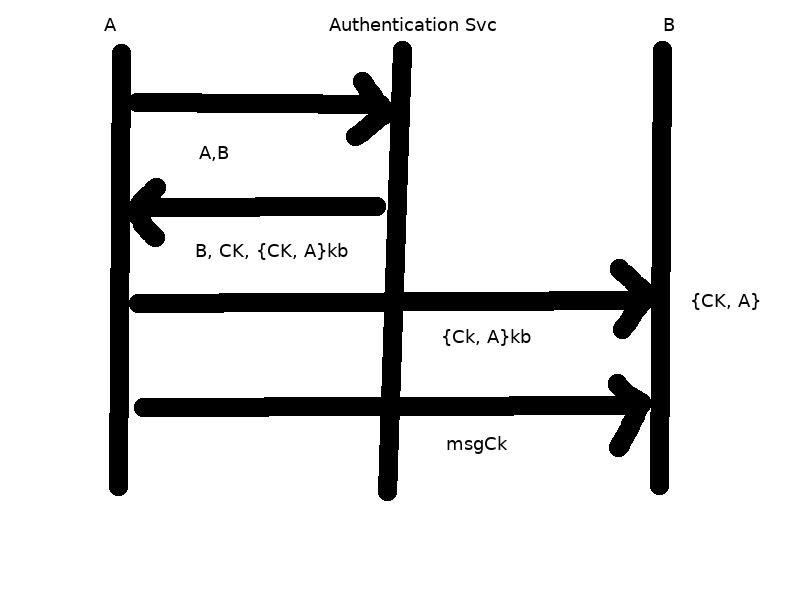
\includegraphics[width=.4\textwidth]{symmetric-key-auth}
                \caption{Symmetric Key Authentication}
                \label{fig:symmetric-key-auth}
            \end{figure}
            \item 
            This is still vulnerable to replay attacks. A nonce (a randomly generated number used only once) can be used to identify such replay attacks, between a sender and an authentication service. For replay attacks to the recipient, a challenge-response approach can be used by `B' to validate that the message originated from A. If B sees messages with a repeated nonce, it discards it.
            \item 
            The above authentication step only occurs once at the start of each session of data transfer. What if an intruder interrupts a session after the authentication is done?\\
            $A \Rightarrow (S_A, S_B, msg) \Rightarrow B$ 
            \item 
            Similar to the challlenge/response phase to validate the authenticity of A, a similar challenge/response will validate the authenticity of B
        \end{itemize}

    % subsection symmetric_key_authentication (end)

    \subsection{Asymmetric Key Authentication} % (fold)
    \label{sub:asymmetric_key_authentication}

        \begin{itemize}
            \item
            Asymmetric authentication. \\
            $A \Rightarrow (S_A, S_B, msg) \Rightarrow B $\\
            where $S_A$ and $S_B$ are monotonically increasing numbers, so that a repeated number can be rejected.\\
            Illustrated in Figure \ref{fig:asymmetric_auth}.
            \begin{figure}[ht]
                \centering
                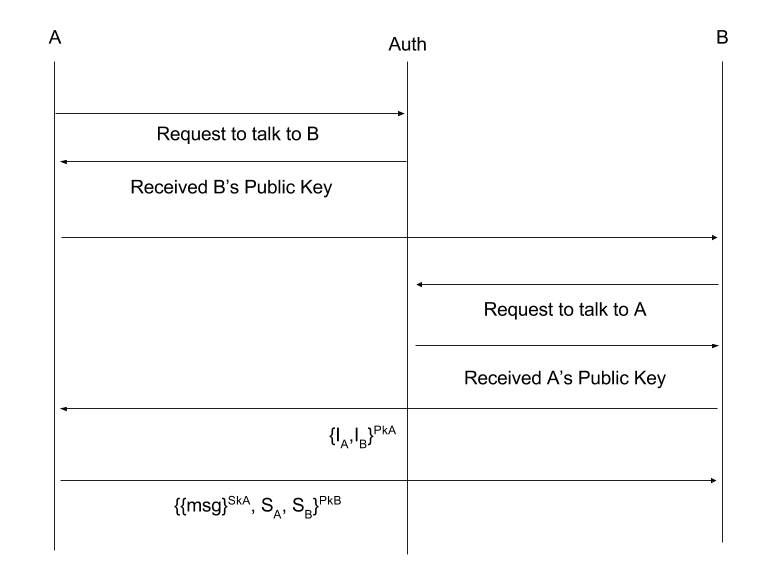
\includegraphics[width=.6\textwidth]{asymmetric_auth}
                \caption{Asymmetric Key Authentication}
                \label{fig:asymmetric_auth}
            \end{figure}
            \item
            Man in the middle attack. Illustrated in Figure \ref{fig:man_in_the_middle_attack}
            \begin{figure}[ht]
                \centering
                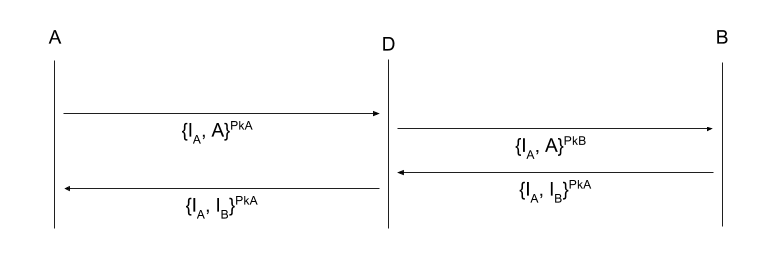
\includegraphics[width=.6\textwidth]{man_in_the_middle_attack}
                \caption{Man-in-the-middle attack}
                \label{fig:man_in_the_middle_attack}
            \end{figure}
        \end{itemize}
    
    % subsection asymmetric_key_authentication (end)

    \subsection{Digital Signatures} % (fold)
    \label{sub:digital_signatures}

        \begin{itemize}
            \item 
            Enforce accountability: no party can deny sending the message
            \item 
            Instead of encrypting the entire message, we compute the hash, and include it while sending, encrypting it with the private key of the sender.\\
            $A \Rightarrow (msg, {hash(msg)}^{SKA}) \Rightarrow B$
        \end{itemize}
    
    % subsection digital_signatures (end)

    \subsection{Asymmetric Auth Design Tips} % (fold)
    \label{sub:asymmetric_auth_design_tips}

        \begin{itemize}
            \item 
            Stateless senders/recipients
            \item 
            Avoid encryption
            \item 
            Reduce authentication service load for scalability, prevention of DoS attacks
        \end{itemize}
    
    % subsection asymmetric_auth_design_tips (end)

% section authentication (end)


\newpage



\section{Scheduling - Sparrow \& Pisces} % (fold)
\label{sec:scheduling}

    \textbf{Goals:}
    \begin{itemize}
        \item 
        High Utilization
        \item 
        Low latency
        \item 
        Fairness - shouldn't prefer one workload over another
        \item 
        Adaptive - 
        \item 
        Support multiple policies - mechanism should be flexible enough to change policies
    \end{itemize}

    \subsection{Sparrow} % (fold)
    \label{sub:sparrow}
        
        \textbf{General Setup}
        \begin{itemize}
            \item 
            Job - composed of small tasks
            \item 
            Set of available workers
            \item 
            Scheduler - assigns the tasks to the workers
        \end{itemize}

        \textbf{Centralized Approach:}\\
        \begin{itemize}
            \item 
            Global information.
            \item 
            Is able to do the best scheduling possible.
            \item 
            Problems:
            \begin{itemize}
                \item 
                Scalability issues - high latency for scheduling
                \item 
                For jobs split into infinitesimally small tasks, the overhead of scheduling might grow larger than the execution time of the task itself.
            \end{itemize}
        \end{itemize}

        \textbf{Decentralized Approach:}\\
        \begin{itemize}
            \item 
            Set of schedulers instead of a single scheduler.
            \item 
            Sparrow's Approaches:
            \begin{itemize}
                \item 
                Random Scheduling - might be effective for low loads, not for higher loads.
                \item 
                Power of 2 choices -  examine 2 nodes, and schedule on the node with the lower workload. Improvement over Random scheduling, but still suffers in the event of high loads.
                \begin{itemize}
                    \item 
                    Optimization 1: Batch probing. For $m$ tasks probe $d*m$ workers, and pick best $m$. This leads to lower latency. 
                    Task queues might be a bad indicator for late
                    \item 
                    Optimization 2: Late binding. Include the probe as a queue message. Broadcast to $2*m$ random nodes. Worker is idle during the pulling step.
                \end{itemize}
            \end{itemize}
        \end{itemize}

        \textbf{Job/Task Constraints:}\\
        \begin{itemize}
            \item 
            Probe the node that meet the constraints.
            \item 
            Per tasks sampling can be done if there are task constraints.
        \end{itemize}

    % subsection sparrow (end)

    \subsection{Pisces} % (fold)
    \label{sub:pisces}

        \begin{itemize}
            \item 
            Provides service guarantees and fairness.
            \item 
            Approaches to segregate services provision
            \begin{itemize}
                \item 
                Resource Partitioning: Assign a portion of the cluster to a specific tenant.\\
                Cons: Low utilization, high cost, coarse grained
                \item 
                Admission Control (centralized scheduler)\\
                Cons: Lack of performance isolation
            \end{itemize}
            \item 
            Each tenant's data is partitioned. Each parition has a different size and a different demand. Each tenant have different request sizes, num. of requests.
        \end{itemize}

        \textbf{Mechanism to serve requests:}
        \begin{itemize}
            \item 
            Mechanism 1: Parition placement should be based on the partition demand.
            \item 
            Mechanism 2: Local weight should match the partition demand, and hence, the partition placement.
            Weight swapping needs to happen as a active part of the system. This includes co-ordination across nodes.
            \item 
            Mechanism 3: Replica selection: Distribute based on relative allocated weights
            \item 
            Mechanism 4: Schedule on dominant resource.
        \end{itemize}

        \textbf{Dominant Resource Fair Sharing}:
        Refer to example in paper
    
    % subsection pisces (end)

% section scheduling (end)


\section{Map-Reduce} % (fold)
\label{sec:map_reduce}

    \textbf{Goal:}
    \begin{itemize}
        \item 
        Perform data-processing at scale.
        \item 
        Efficiently use all the available nodes.
        \item 
        Handle failures
    \end{itemize}

    \textbf{Overview:}
    \begin{itemize}
        \item 
        Divide work into sub-tasks
        \item 
        Run sub-tasks independently
        \item 
        If a sub-task fails, then re-do
    \end{itemize}

    \textbf{Programming Model:}
    \begin{itemize}
        \item 
        Mapper: $Map(K,V) \Rightarrow (K\prime, V\prime) ... emit(K\prime, V\prime)$
        \item 
        Reduce: $Reduce(Result, Iterator(K)) ... emit(Result)$
        \item 
        Example of word count MR program.
    \end{itemize}

    \textbf{Implementation}
    \begin{itemize}
        \item 
        Illustration: Figure \ref{fig:mapreduce-implementation}
        \begin{figure}[ht]
            \centering
            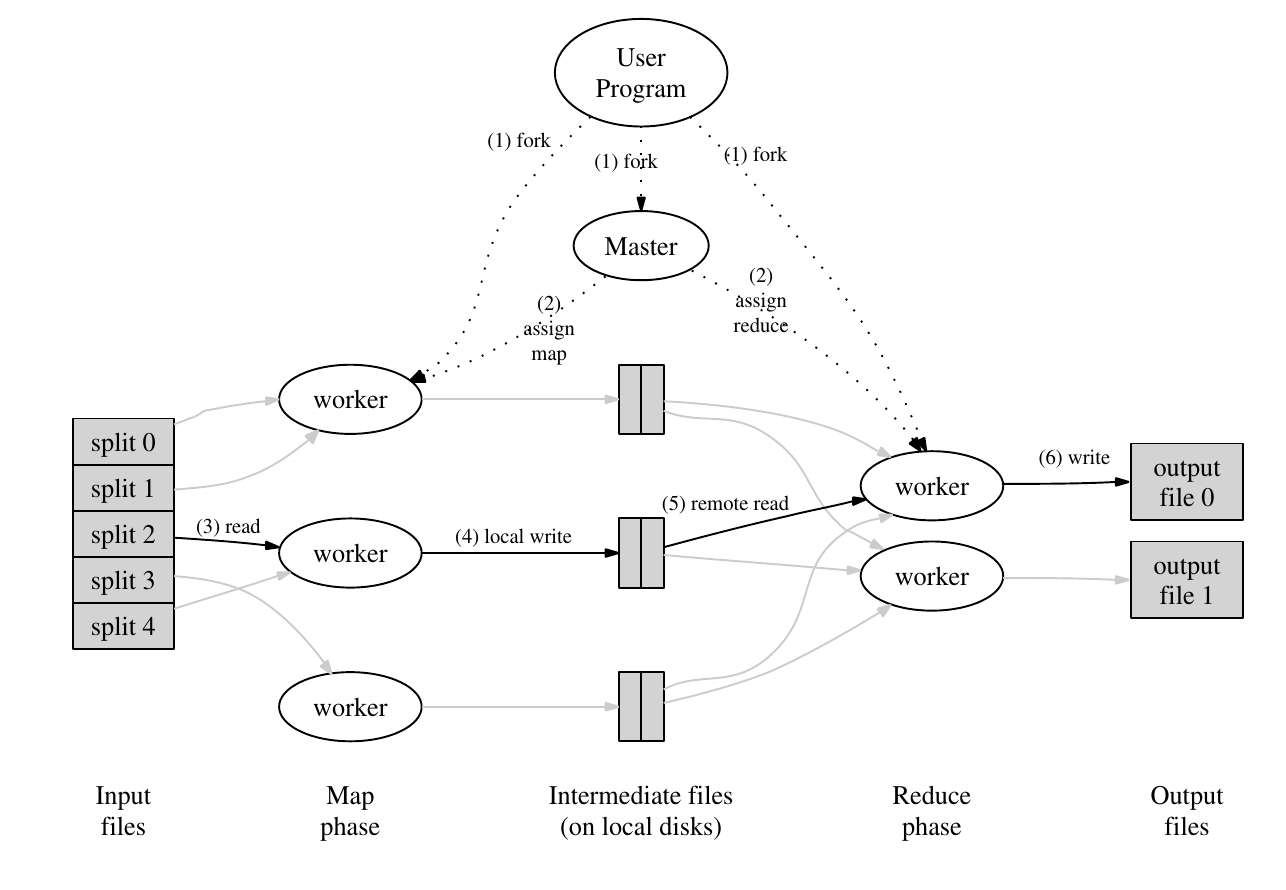
\includegraphics[width=\textwidth]{mapreduce-implementation}
            \caption{Map-Reduce Implementation}
            \label{fig:mapreduce-implementation}
        \end{figure}
        \item 
        The input and results are stored on GFS, which is ditributed and consistent.
        \item 
        Intermediate results are stored locally. These are stored as small files.
        \item 
        2 phases
        \begin{itemize}
            \item 
            Phase 1:
            \begin{itemize}
                \item 
                Map re-distributed data
            \end{itemize}
            \item 
            Phase 2:
            \begin{itemize}
                \item 
                Sort
                \item 
                Reduce
                \item 
                Write results to GFS
            \end{itemize}
        \end{itemize}
    \end{itemize}

    \textbf{Fault Tolerance:}
    \begin{itemize}
        \item 
        Master: Redo the task
        \item 
        Worker:
        \begin{itemize}
            \item 
            Master uses a monitor on the worker
            \item 
            Re-schedule the sub-task on a new node
        \end{itemize}
    \end{itemize}

    \textbf{Locality:}
    Schedule tasks on mapper nodes that already have the input file required for the computation.

    \textbf{Stragglers:}
    \begin{itemize}
        \item 
        Slow nodes become a bottleneck for the entire MR job
        \item 
        Create backup tasks, whichever finishes first will have their results chosen
    \end{itemize}

% section map_reduce (end)


\section{Google File System} % (fold)
\label{sec:google_file_system}

    \textbf{Assumptions:}
    \begin{itemize}
        \item 
        Failures are common
        \item 
        Fewer, larger files
        \item 
        Mostly sequential I/O access. Writes are mostly appends
        \item 
        Bandwidth is prioritized over latency for Google workloads
    \end{itemize}

    \textbf{Interface:}
    \begin{itemize}
        \item 
        Open
        \item 
        Read
        \item 
        Write/append
        \item 
        Close
    \end{itemize}

    \textbf{Architecture:}
    \begin{itemize}
        \item 
        Illustration: Figure \ref{fig:gfs-architecture}
        \begin{figure}[ht]
            \centering
            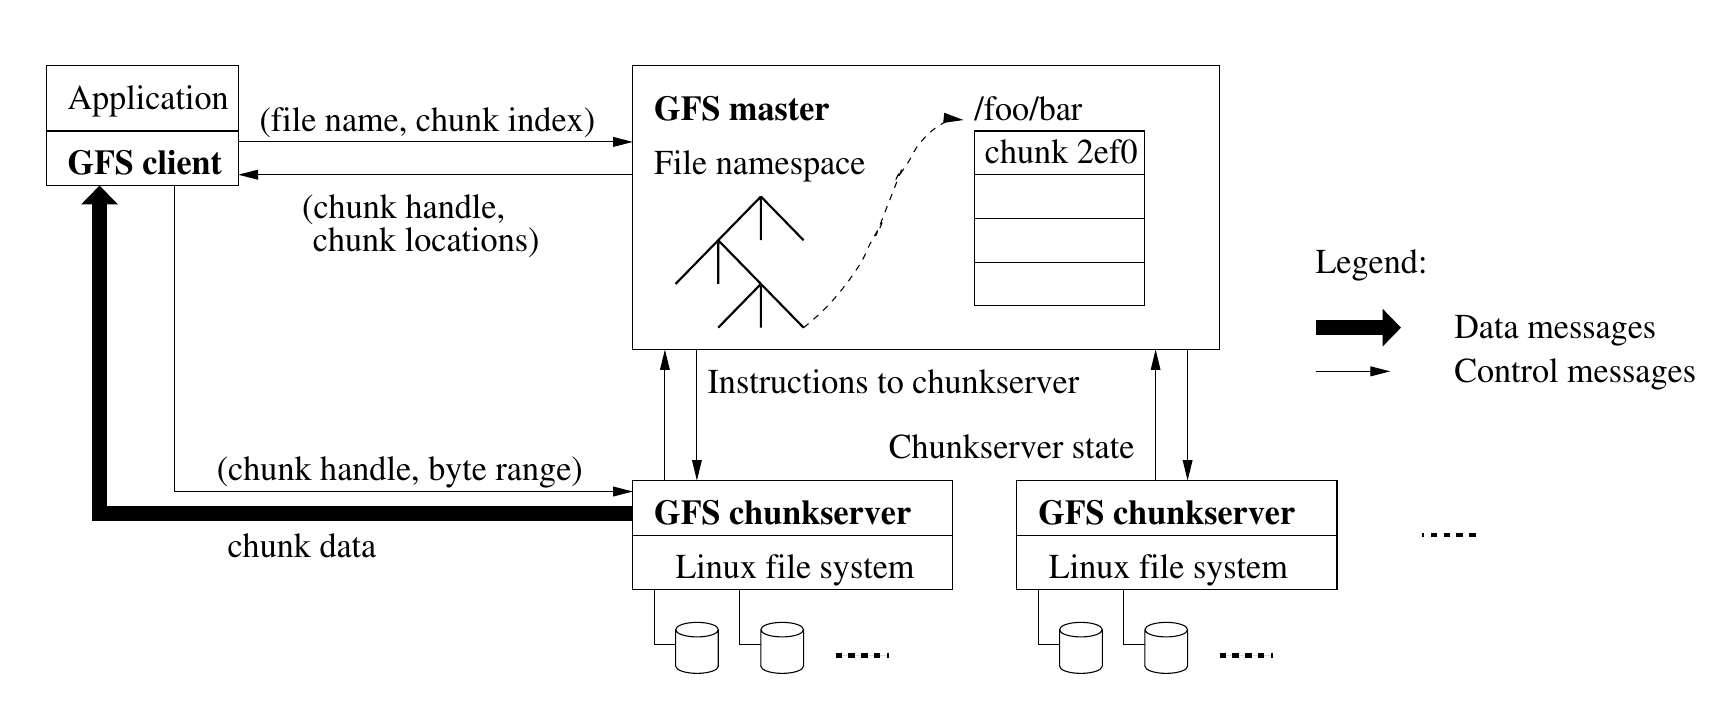
\includegraphics[width=.8\textwidth]{gfs-architecture}
            \caption{GFS Architecture}
            \label{fig:gfs-architecture}
        \end{figure}
        \item 
        Single Master
        \item 
        Chunkservers (files are chunked into 64MB chunks). This reduces metadata overhead and big data movement.
        \item 
        Multiple clients
    \end{itemize}

    \textbf{Metadata:}
    \begin{itemize}
        \item 
        File namespace
        \item 
        Mapping file $\Rightarrow$ chunks
        \item 
        Logged and Replicated
        \item 
        Identifiers for the chunkservers are not persisted on the metadata node, it's built in-memory.
        \item 
        Since the chunks across multiple node are very large in number, this results in a slow bootstrap time for GFS.
    \end{itemize}

    \textbf{Write protocol:}
    \begin{itemize}
        \item 
        Illustration: Figure \ref{fig:gfs-write-protocol}
        \begin{figure}[ht]
            \centering
            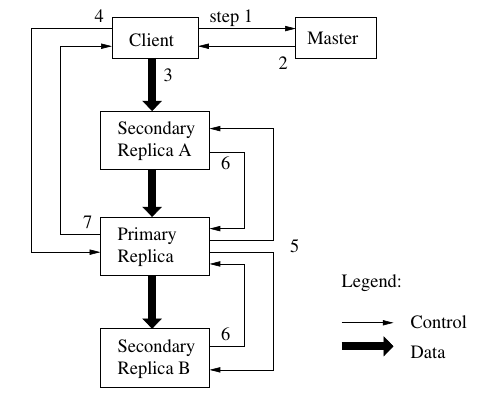
\includegraphics[width=.6\textwidth]{gfs-write-protocol}
            \caption{GFS Write Protocol}
            \label{fig:gfs-write-protocol}
        \end{figure}
        \item 
        Serialize updates 
        \begin{itemize}
            \item 
            Master gives a lease to a `primary' chunk
            \item 
            Primary does the ordering of the updates
        \end{itemize}
        \item 
        Append operation is atomic. And the guarantee of GFS is that the append is done `at least once'
        \item 
        Application should handle duplicate records
    \end{itemize}

% section google_file_system (end)


\newpage


\section{Facebook Tao} % (fold)
\label{sec:facebook_tao}

    \begin{itemize}
        \item 
        The main system for rendering FB.
        \item 
        Workload  99.8\% reads and 0.2\% writes.
        \item 
        Single global instance of TAO running at FB.
        \item 
        Most data is old and cold.
        \item 
        Hundreds of reads per client.
        \item 
        Eventually consistent. 
    \end{itemize}

    \textbf{Data Model:}
    \begin{itemize}
        \item 
        Best expressed as a graph.
        \item 
        Nodes include users, posts, comments
        \item 
        Objects:
        $id \Rightarrow type, (key, value)$
        \item 
        Association:
        $(id1, atype, id2) \Rightarrow time, (key, value) $
        \item 
        Association list: (query limit is capped - pagination)
        $id, atype: [newest .. oldest]$
    \end{itemize}

    \textbf{Consistency Model:}
    \begin{itemize}
        \item 
        Eventually consistent, with read-my-writes from the same web-server.
    \end{itemize}

    \textbf{System Architecture:}
    \begin{itemize}
        \item 
        Data stored on sharded MySQL instances
        \item 
        Stateless caching nodes.
        \item 
        Each web server talks to a subset of follower caches
    \end{itemize}

    \textbf{Caching:}
    \begin{itemize}
        \item 
        Issues with single-layer caching:
        \begin{itemize}
            \item 
            Order writes
            \item 
            Invalidate/refill caches
            \item 
            Reduce hot-spots on MySQL
        \end{itemize}
    \end{itemize}

    \textbf{Handling Writes:}
    \begin{itemize}
        \item 
        Write to MySQL
        \item 
        Leader sends a refill msg to all followers (The advantage of doing this is that it is scalable, as we don't need to maintain a list of which follower cache has what data.)
        \item 
        Followers who cache `X' will refill
        \item 
        Caching protocol is idempotent.
    \end{itemize}

    \textbf{Writes across Data Centers:}
    \begin{itemize}
        \item 
        Master Data center for each shard, and replica data centers
        \item 
        When a leader receives a write request for a record which isn't sharded locally the leader cache sent the data to the master data center's leader.
    \end{itemize}

% section facebook_tao (end)


\section{Google Spanner} % (fold)
\label{sec:google_spanner}

    \begin{itemize}
        \item 
        Global consistent storage, with lock-free reads
        \item 
        Snapshots of the data to provide lock-free reads        
        \item 
        Reads can be done from objects at multiple snapshots. The snapshots must remain consistent i.e. made at the same time.
        \item 
        External consistency: Order of commits are the same as the order visible to the user.
        \item 
        How is this acheived?
        \begin{itemize}
            \item 
            Writes are timestamped
            \item 
            Issues with timestamps are network delay and time drifts
            \item 
            Use a global clock
        \end{itemize}
    \end{itemize}

    \textbf{True Time:}
    \begin{itemize}
        \item 
        API to provide the global clock.
        \item 
        $TT.now$ yields a range, not an absolute value
        \item 
        Wait out uncertainty
    \end{itemize}


% section google_spanner (end)


\end{document}
